\usepackage{extras}
\usetheme{default}
\usecolortheme{dove}

\title{Konstruktion av en autonom undsättningsrobot}
\subtitle{Kandidatprojekt i elektronik vid Linköpings universitet}
\author{Grupp 4}
\beamertemplatenavigationsymbolsempty
\date{\today}

\begin{document}

\begin{frame}
  \titlepage
\end{frame}


\begin{frame}{PigBot}{Grupp 4}
  \begin{columns}
    \begin{column}{0.5\textwidth}
      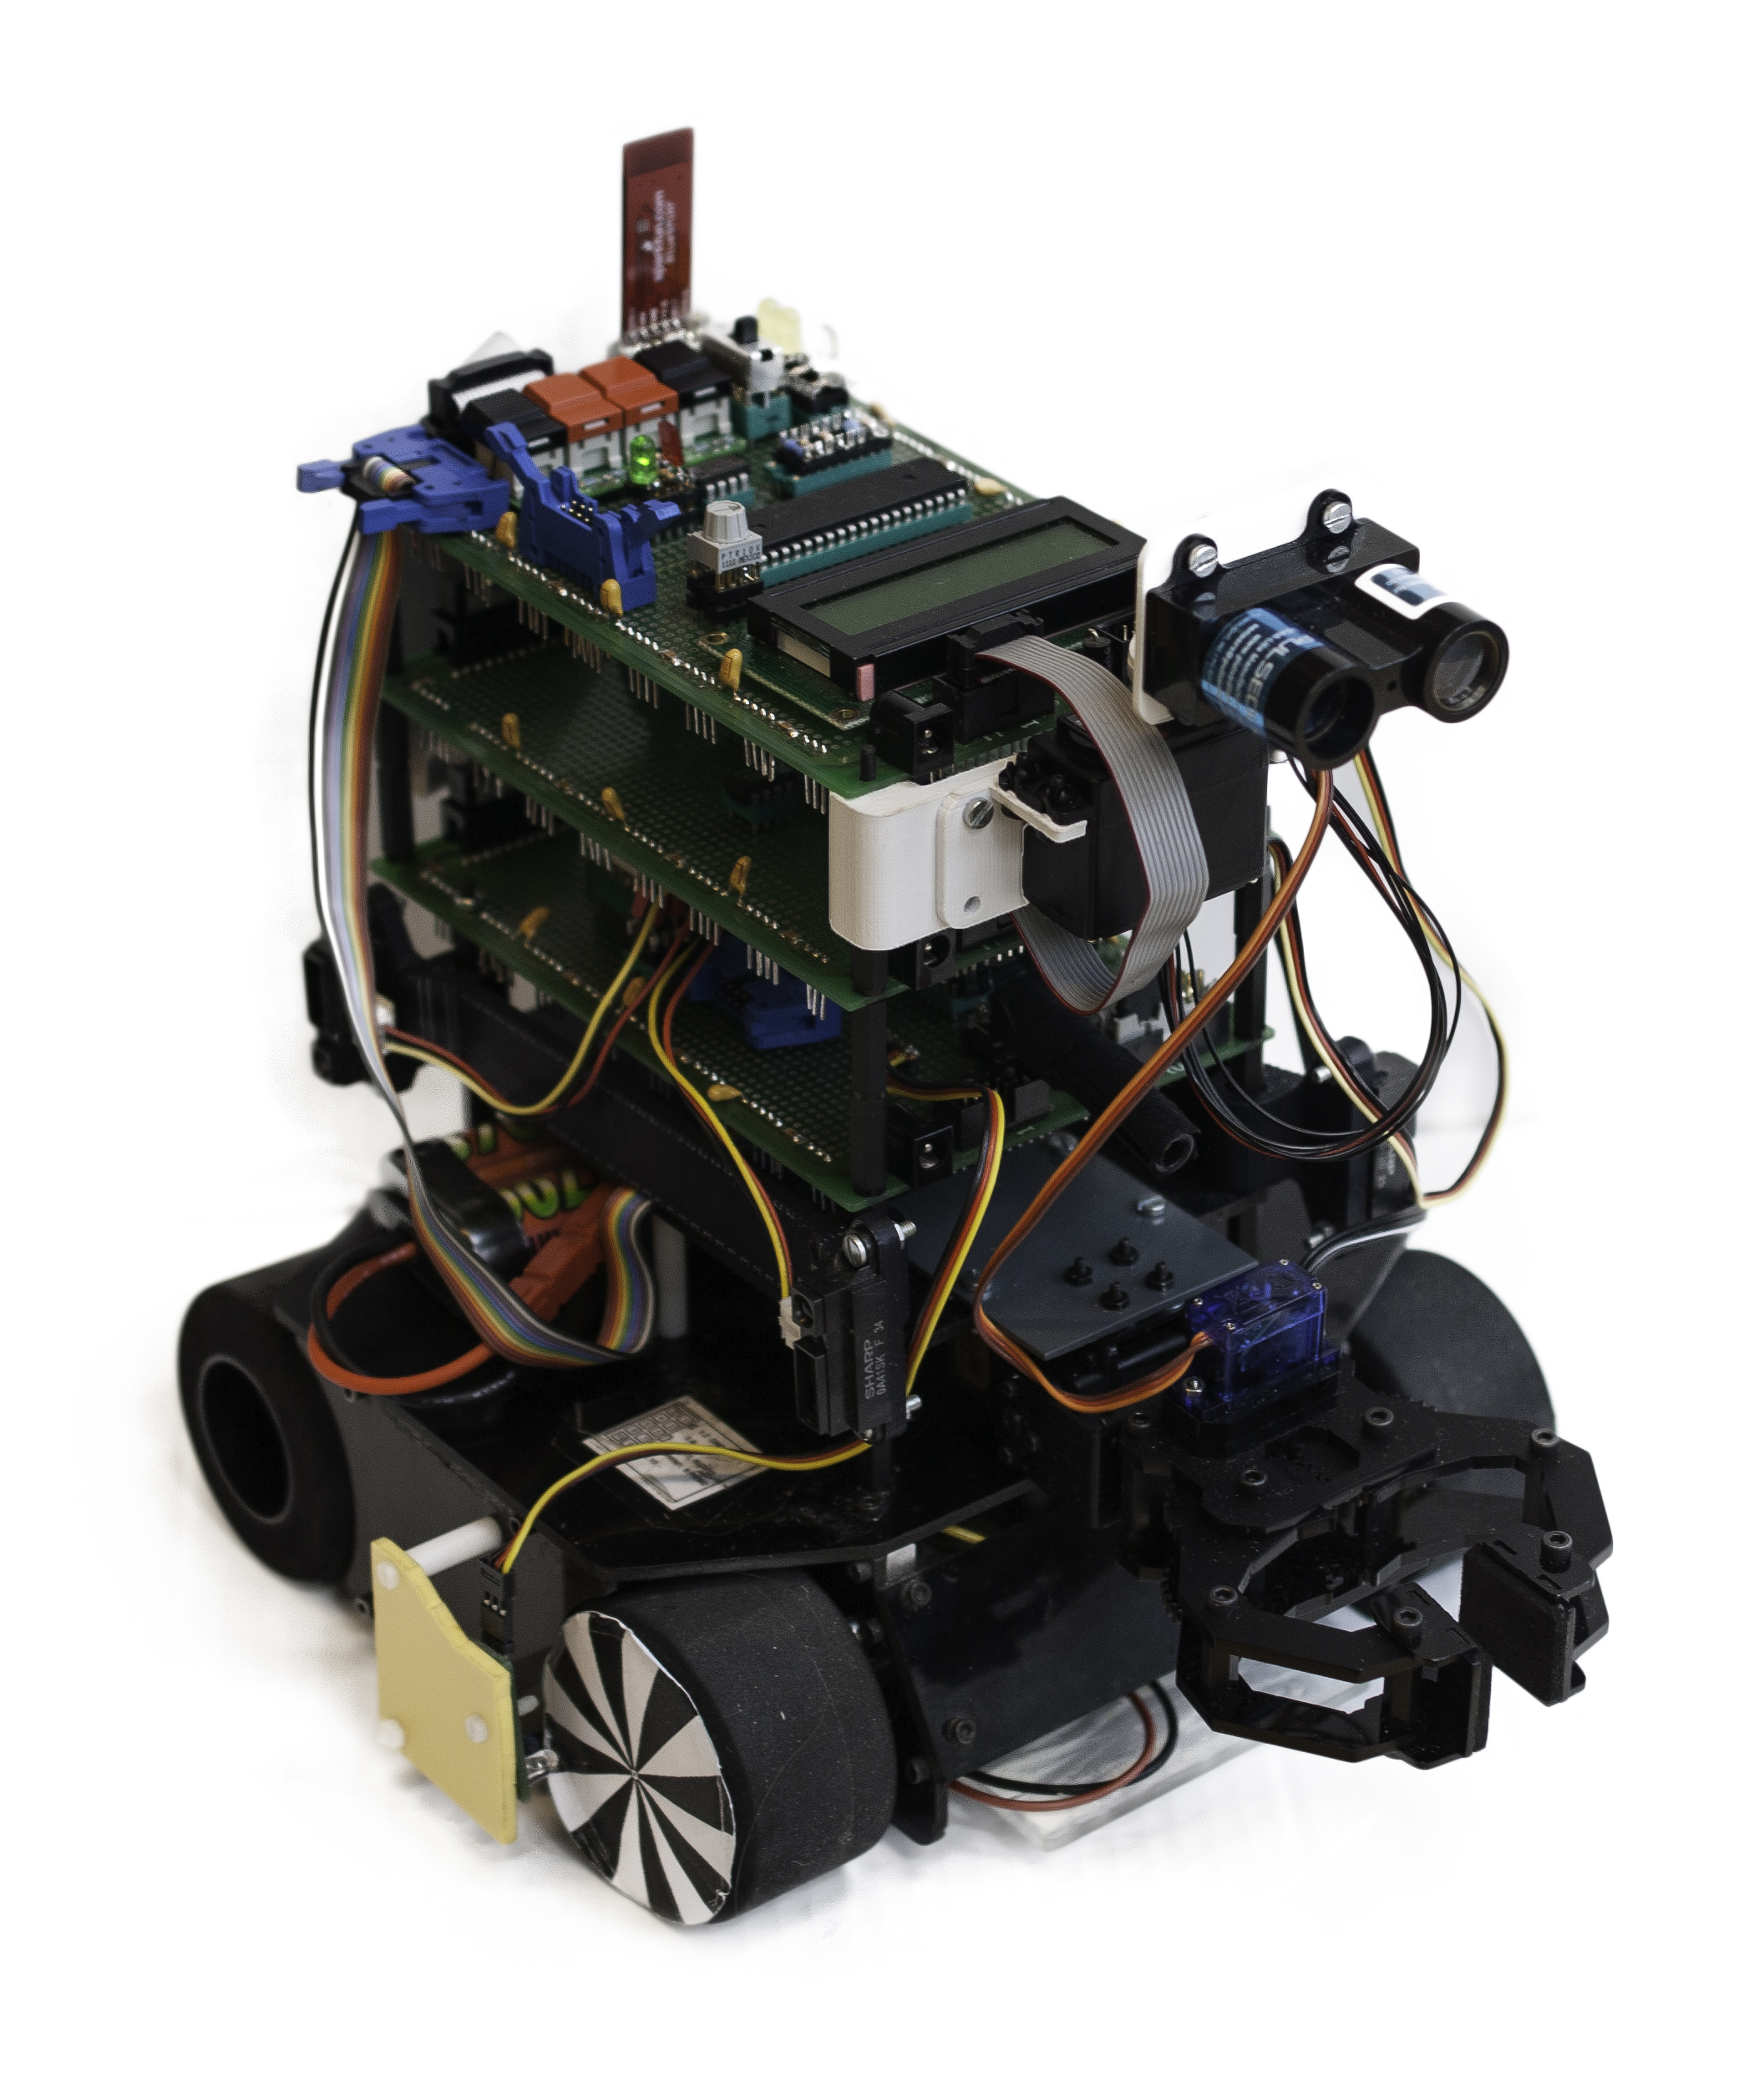
\includegraphics[width=0.9\textwidth]{images/RobotFront.pdf}
    \end{column}
    \begin{column}{0.5\textwidth}
      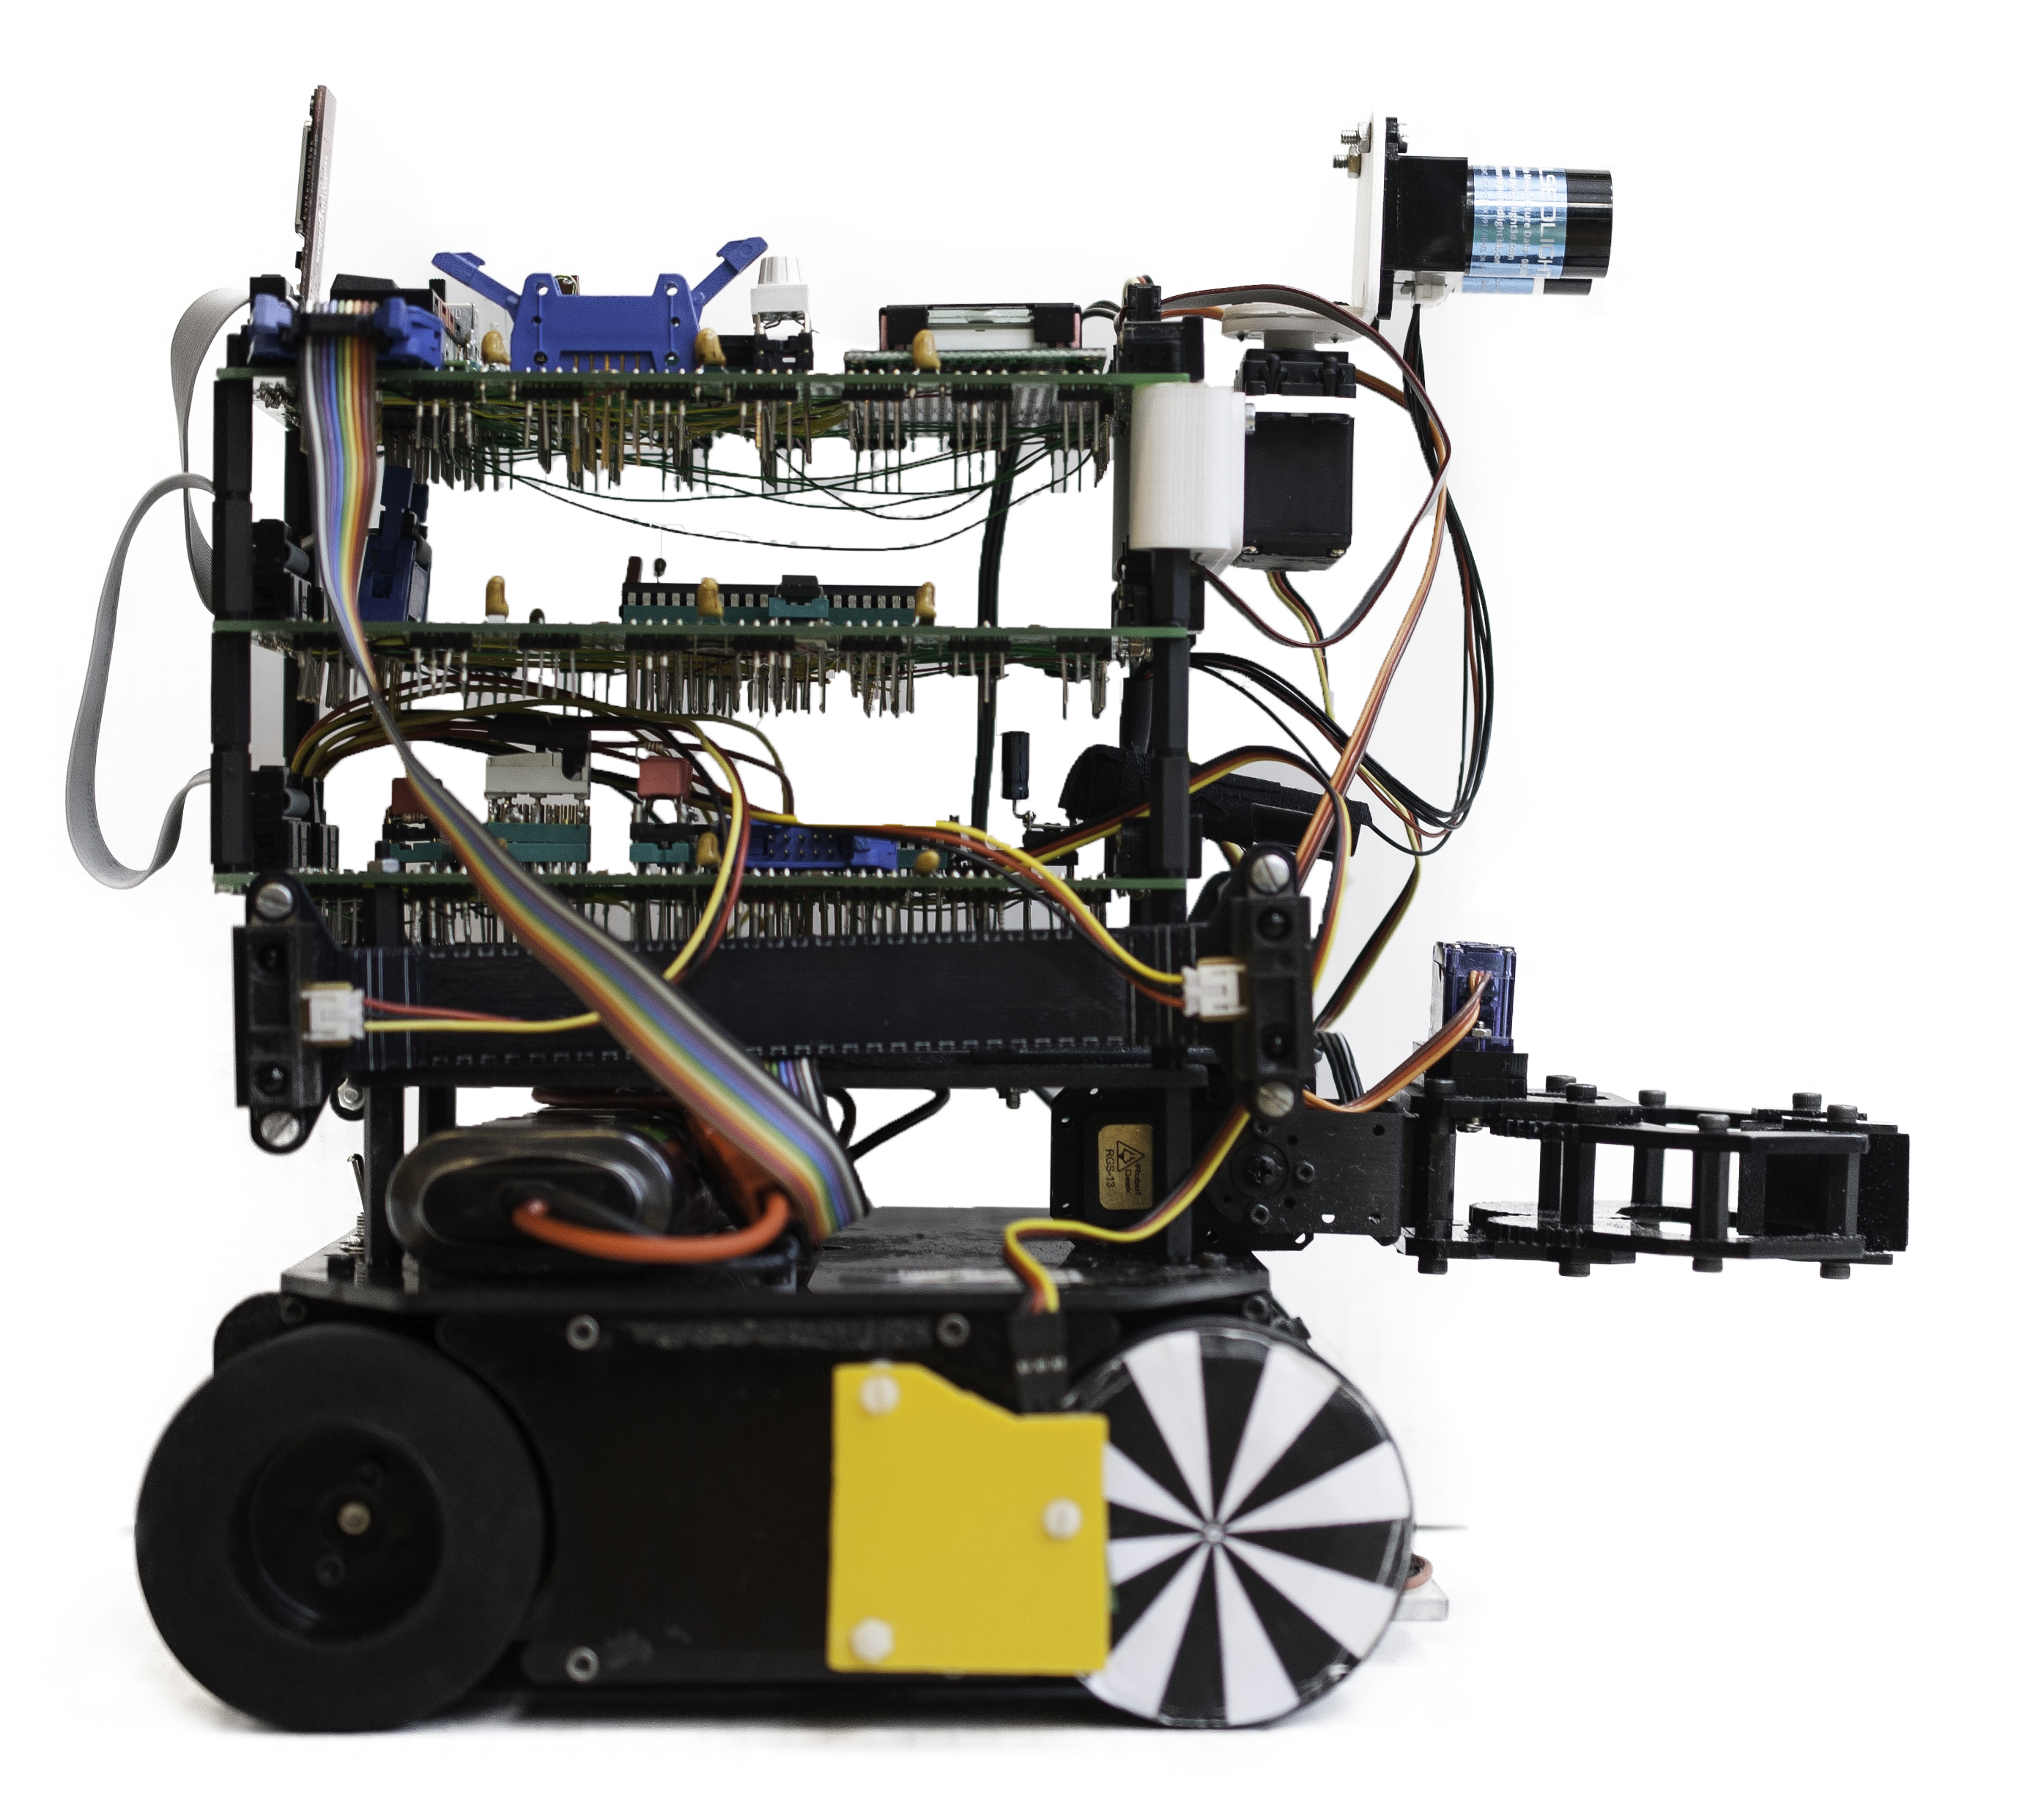
\includegraphics[width=\textwidth]{images/RobotSide.pdf}
    \end{column}
  \end{columns}
\end{frame}

\begin{frame}[fragile]{PigBot}{Grupp 4}
Syfte och uppgift:
\pause
  \begin{itemize}
    \item[-] Undsättningsrobot på prototypnivå
\pause
    \item[-] Utforskar autonomt ett simulerat grottsystem
\pause
    \item[-] Identifierar och undsätter en nödställd
\pause
    \item[-] Kommunicerar kartdata till extern dator via Bluetooth\textsuperscript{\circledR}


  \end{itemize}
\end{frame}

\begin{frame}[fragile]{PigBot}{Grupp 4}
\centering
    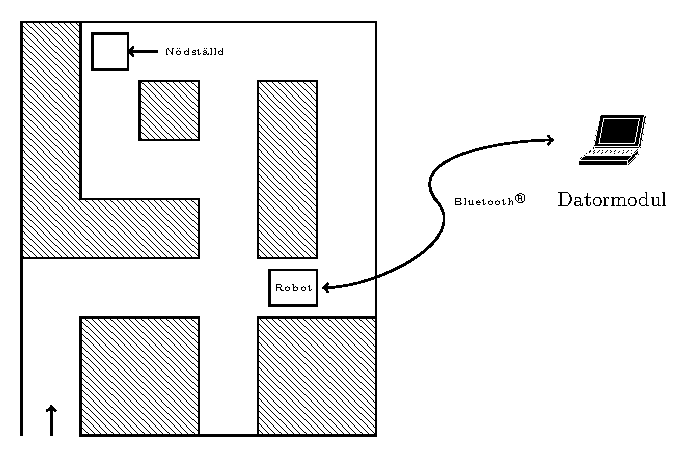
\includegraphics[scale=0.7]{images/overview.pdf}

\end{frame}

\begin{frame}[fragile]{PigBot}{Grupp 4}

PigBot är upbyggd av moduler, vardera med följande funktion:
  \begin{itemize}
\pause
    \item[-] Sensormodul - tar emot och koverterar data från robotens samtliga sensorer
\pause
    \item[-] Styrmodul - sköter reglering av roboten och rotation av roboten samt skriver ut sensordata till en LCD-display
\pause
    \item[-] Huvudmodul - Upprättar kommunikationen via Bluetooth\textsuperscript{\circledR} för att kommunicera kartdata
  \end{itemize}
\end{frame}

% Olles del
\begin{frame}{PigBot}{Grupp 4} 
  \begin{columns}
    \begin{column}{0.5\textwidth}
      \centering
      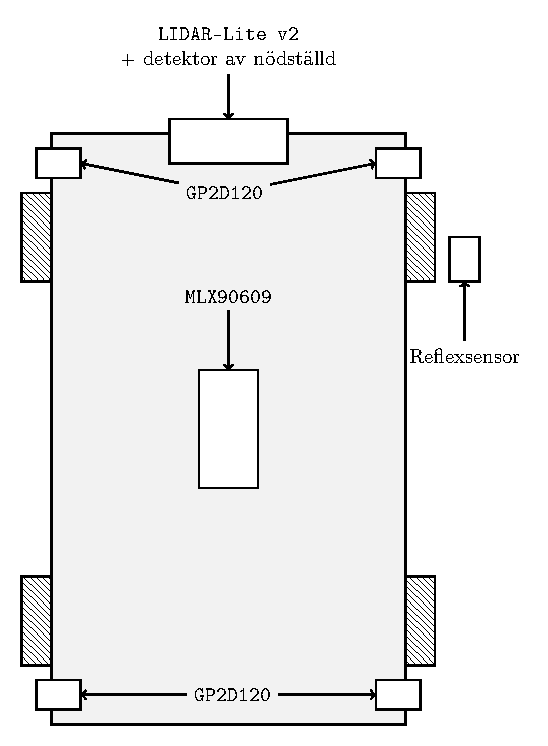
\includegraphics[scale=0.6]{images/sensor.pdf}
    \end{column}
    \begin{column}{0.5\textwidth}

      Sensormodul
      \begin{itemize}
	\item[-] Åtta sensorer
	  \begin{itemize}
	    \item[-] Fyra sidosensorer (IR)
	    \item[-] En främre sensor (laser)
	    \item[-] En reflexsensor (IR)
	    \item[-] Ett gyroskop (SPI)
	    \item[-] En måldetektor (IR)
	  \end{itemize}
	  \pause
	\item[-] Beräknar median efter sampling
	  \pause
	\item[-] Skickar vidare i $30$ Hz
      \end{itemize}
    \end{column}

  \end{columns}
\end{frame}

\begin{frame}{PigBot}{Grupp 4}
  Huvudmodul
  \begin{center}
    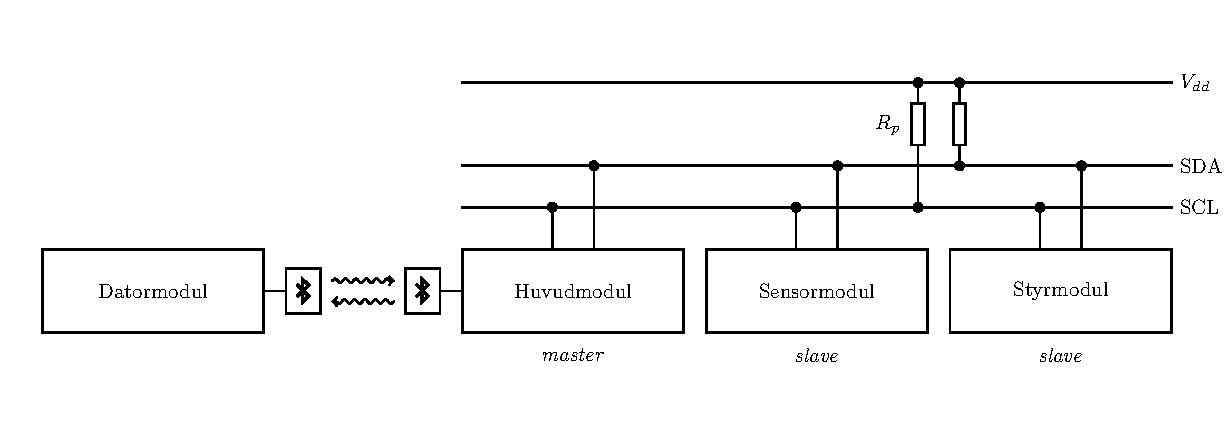
\includegraphics[scale=0.5]{images/communication.pdf} 
    \pause
    \begin{longtable}{c c c c c}
      {Identifierare} & & {Kommando} & & {Data} \\ \hline
      246-255 & $\rightarrow$ & 0-245 & $\rightarrow$ & 0-245 
    \end{longtable}
  \end{center}
\end{frame}

% Isaks del
\begin{frame}{PigBot}{Grupp 4}
	\begin{columns}
		\begin{column}{0.5\textwidth}
			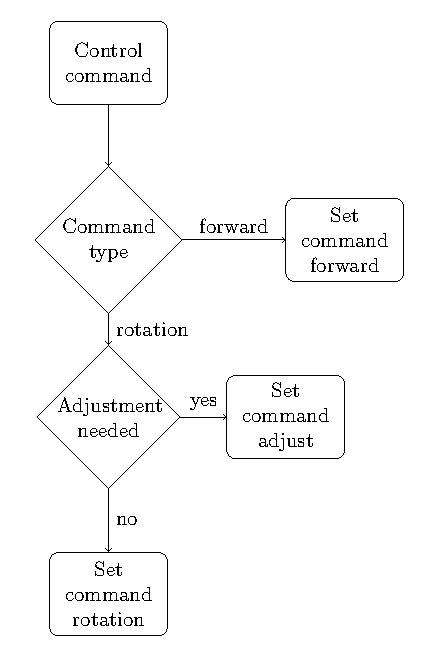
\includegraphics[width=0.9\textwidth]{images/controllerControlFlow.pdf}
		\end{column}
		\pause
    		\begin{column}{0.5\textwidth}
      			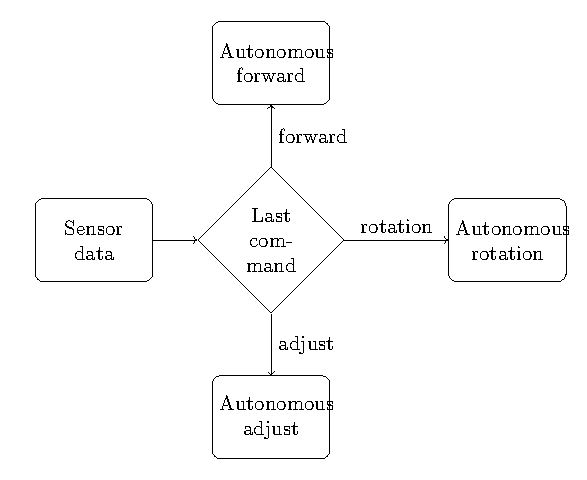
\includegraphics[width=\textwidth]{images/controllerSensorFlow.pdf}
    		\end{column}
  	\end{columns}
\end{frame}

\begin{frame}{PigBot}{Grupp 4}
\centering
	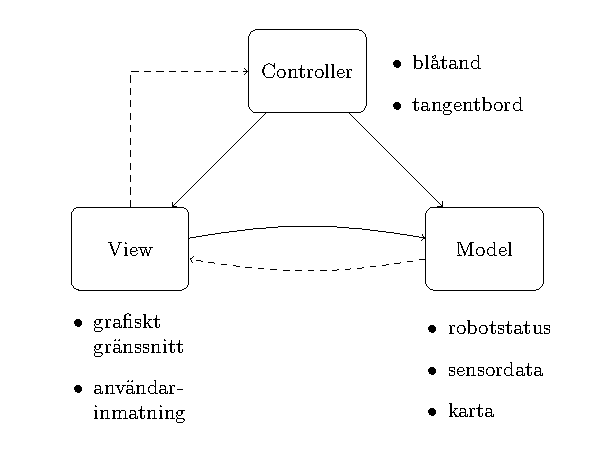
\includegraphics[width=0.9\textwidth]{images/modelViewController.pdf}
\end{frame}

\begin{frame}{PigBot}{Grupp 4}
	\begin{tikzpicture}[scale=0.135]
		\pgftext{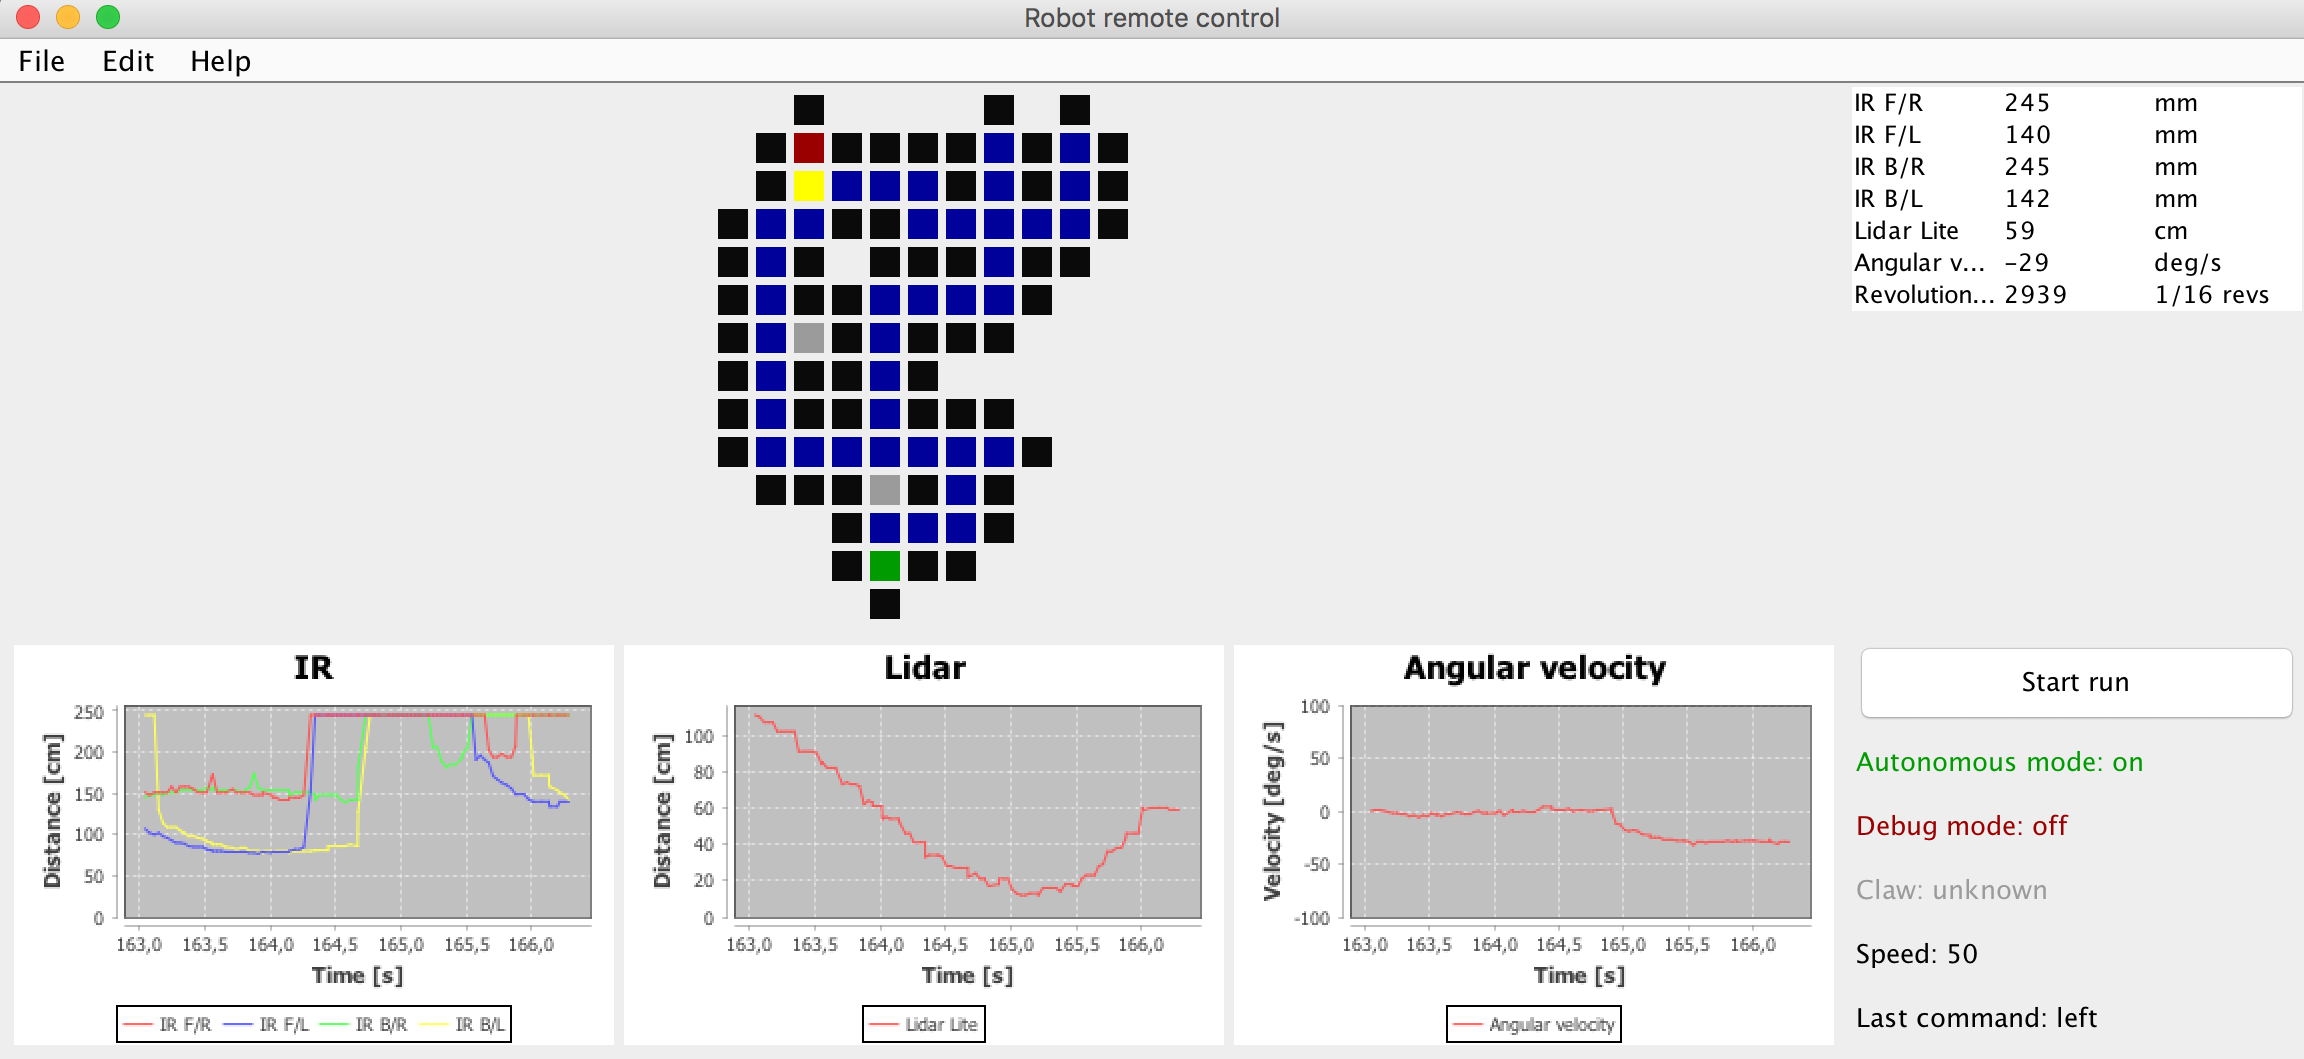
\includegraphics[width=2304pt]{images/computerModule.png}} at (0pt,0pt);
		\fill<3-6>[black, opacity = 0.7] (-1150 pt, 527pt) rectangle (1150pt , 450pt);
		\fill<2, 4-6>[black, opacity = 0.7] (-1150pt, 450pt) rectangle (700pt , -100pt);
		\fill<2-4, 6>[black, opacity = 0.7] (-1150pt, -100pt) rectangle (700pt , -527pt);
		\fill<2-3, 5-6>[black, opacity = 0.7] (700pt, 450pt) rectangle (1150pt , -100pt);
		\fill<2-5>[black, opacity = 0.7] (700pt, -100pt) rectangle (1150pt , -527pt);
	\end{tikzpicture}
\end{frame}

% Avslutning och skryt
\begin{frame}[fragile]{PigBot}{Grupp 4}
Resultat
  \begin{itemize}
\pause
    \item[-] Roboten PigBot
\pause
    \item[-] Prestanda
  \end{itemize}
\end{frame}

\begin{frame}[fragile]{PigBot}{Grupp 4}
  \begin{itemize}
    \item[-] Eventuell animation 
  \end{itemize}
\end{frame}

\begin{frame}[fragile]{PigBot}{Grupp 4}
Utvecklingspotential 
  \begin{itemize}
 \pause
    \item[-] Optimera avsökningsalgoritm
 \pause
    \item[-] Göra mer verklighetsanpassad
	\begin{itemize}
	  \item Öppna ytor
	  \item Rotation
	\end{itemize}	
  \pause
    \item[-] Förbättra användarupplevelsen
     	\begin{itemize}
	  \item 3D-karta
	\end{itemize}
   \end{itemize}
\end{frame}


\begin{frame}[fragile]{PigBot}{Grupp 4}
Hur gruppen har jobbat:
  \begin{itemize}
 \pause
    \item[-] Gruppkontrakt 
\pause
    \item[-] Paruppdelning
\pause
    \item[-] Bestämda mötestider
\pause
    \item[-] Tid och plats
\pause
    \item[-] Umgänge utanför arbetstid
  \end{itemize}
\end{frame}

\begin{frame}[fragile]{PigBot}{Grupp 4}
Problemlösning
  \begin{itemize}
 \pause
    \item[-] Situationsanpassat
\pause
    \item[-] Exempel
  \end{itemize}
\end{frame}

\begin{frame}[fragile]{PigBot}{Grupp 4}
Konflikter
  \begin{itemize}
 \pause
    \item[-] Kommunikation
\pause
    \item[-] Ansvar
  \end{itemize}
\end{frame}

\begin{frame}[fragile]{PigBot}{Grupp 4}
Avslutning \& skryt
  \begin{itemize}
 \pause
    \item[-] Beror på vad ni andra har tagit upp
  \end{itemize}
\end{frame}

\end{document}
